In order to enhance the user experience of the authentication and authorisation
mechanism described in \Cref{sub:backend_auth}, the application utilises local
storage to store the user id. This approach provides a seamless and persistent
user experience by retaining the user's identification information across
sessions. The flowchart depicting the logic of this process is presented in
\Cref{fig:frontend_auth_state}.

\begin{figure*}[!htb]
  \caption{User ID storage Flowchart}
  \label{fig:frontend_auth_state}
  \centering
  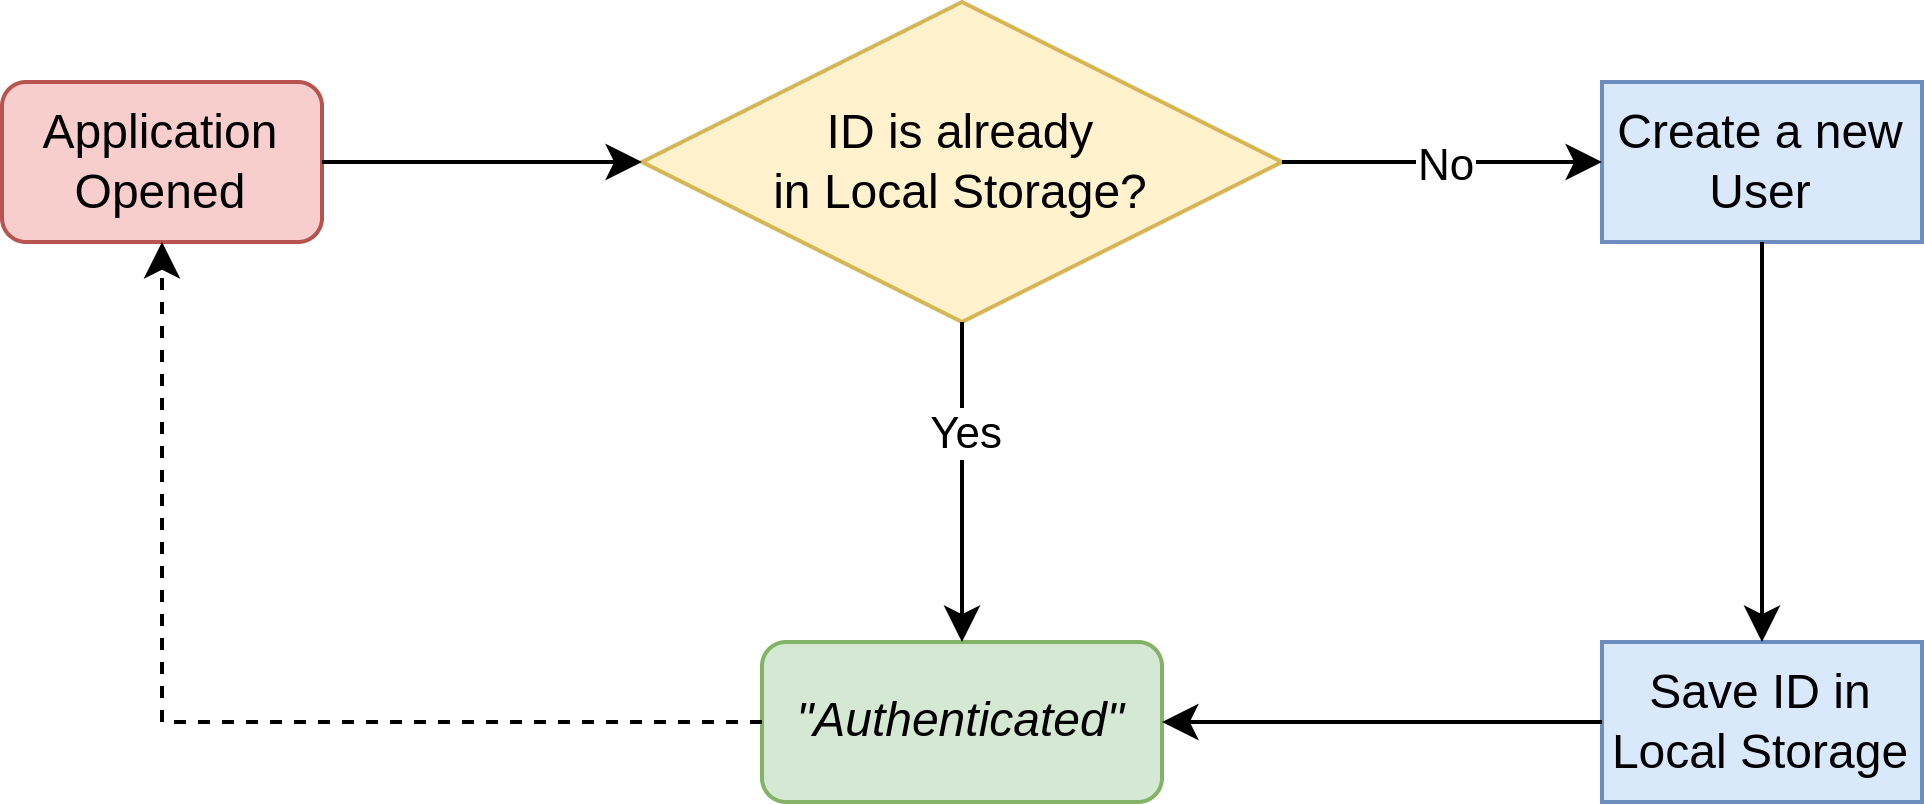
\includegraphics[width=\textwidth]{thesis-frontend_auth_state.drawio}
\end{figure*}

However, it is essential to note that users can manually remove their user id
from local storage. This action carries the risk of losing access to all their
previous decompositions. Therefore, users should exercise caution when manually
deleting their user id, as it may result in losing important data and restrict
their access to previous work within the application.
